\documentclass{article}
\usepackage[utf8]{inputenc}
\usepackage[spanish]{babel}
\usepackage{amsmath}
\usepackage{amsfonts}
\usepackage{amssymb}
\usepackage{graphicx}
\usepackage[left=2cm,right=2cm,top=2cm,bottom=2cm]{geometry}
\usepackage{listings}
\usepackage[hidelinks]{hyperref}

\lstset {
    frame = single,
    breaklines = true
}



\begin{document}

\begin{titlepage}
\title{\textbf{
    {\Huge Práctica 6: Pentesting de aplicaciones Web}\\
    {\Large Seguridad Informática}
}}
\author{
    Pedro Allué Tamargo (758267)
    \and
    Juan José Tambo Tambo (755742)
}
\date{\today}
\clearpage\maketitle
\thispagestyle{empty}
\tableofcontents
\end{titlepage}


\section{Ataque \textit{SQLi}}

Con este ataque se pretende inyectar código \textit{SQL} en el servidor utilizando un formulario. El objetivo de este ataque es conseguir la contraseña de todos los usuarios del sistema.\\


\subsection{Nivel bajo}
%Obtención del user 3: 
%\begin{lstlisting}
%a' UNION SELECT first_name, last_name FROM users WHERE user_id = 3; #
%\end{lstlisting}

Para la explotación de esta vulnerabilidad se va introducir el siguiente texto en el formulario:

\begin{lstlisting}
a' UNION SELECT first_name, password AS last_name FROM users; #
\end{lstlisting}

El código que procesa la petición de este formulario no comprueba los valores que se utilizan en la variable \texttt{id}. Por lo tanto se utilizará una sentencia \textit{UNION} para concatenar el resultado de la consulta con el resultado otra consulta que devuelve el nombre y la contraseña \textit{hasheada} (utilizando el algoritmo \textit{md5}) del usuario en el campo \textit{last\_{}name}.\\
El resultado de la explotación de esta vulnerabilidad se puede observar en la Figura \ref{fig:sql_injection_low}. Se puede observar que la contraseña está codificada utilizando el algoritmo \textit{md5} ya que la contraseña del usuario \textit{admin} es \textit{password} y utilizando este algoritmo se codifica como: \texttt{5f4dcc3b5aa765d61d8327deb882cf99}\footnote{\url{https://www.md5hashgenerator.com/}}.\\

\begin{figure}[h!]
    \centering
    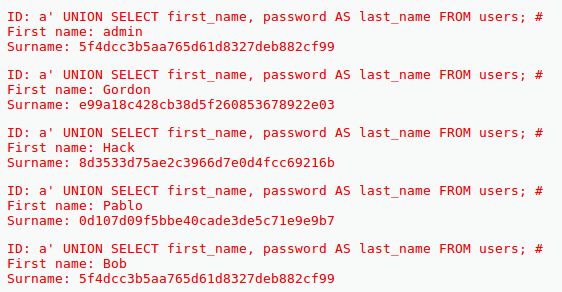
\includegraphics[scale=0.8]{images/sql_injection_password_hash.png}
    \caption{Captura de pantalla del resultado de la ejecución de la sentencia mostrada}
    \label{fig:sql_injection_low}
\end{figure}


\subsection{Nivel medio}
\label{section:sqli_medium}

El nivel intermedio se compone de un formulario utilizando un componente \textit{dropdown}, es decir, los valores están predefinidos por defecto y no se pueden modificar. Otro cambio observable en el código de la aplicación es que ahora la petición es de tipo \texttt{POST}, lo que significa que los parámetros están codificados en el cuerpo del mensaje y no en la \textit{URL}.\\
Por lo tanto para interaccionar con las peticiones se deberá utilizar alguna herramienta adicional para cambiar el contenido de la petición o enviar peticiones al servidor utilizando el método \textit{POST}.\\

Se va a utilizar la herramienta \textit{ZAP (Zed Attack Proxy)}. Esta herramienta funciona como un \textit{Proxy} que monitoriza las peticiones desde el navegador al servidor. Se ha actualizado la versión encontrada en la máquina virtual a la versión \textit{2.9.0} para tener acceso a la herramienta \textit{ZAP HUD} que está disponible a partir de la versión \textit{2.8.0}. No obstante se han encontrado problemas a la hora de utilizar esta herramienta ya que el navegador (\textit{Firefox}) no era capaz de cargar el contenido de la misma.\\
No obstante se ha conseguido interceptar el tráfico de la aplicación y sus peticiones hacia el servidor. Una vez interceptada una petición \textit{POST} se pueden obtener los valores como la \textit{cookie} y el contenido del mensaje. Si se selecciona el mensaje y se utiliza la opción \textit{``Resend with...''} se puede modificar el cuerpo del mensaje. Si se añade el siguiente código se puede explotar la vulnerabilidad.

%Ahora es un post y un formulario más cerrado... Usaremos la herramienta \textit{OWASP ZAP (Zed Attack Proxy)}.\\
%Se ha tenido que actualizar ZAP a la versión más reciente para tener un interfaz gráfico para atacar con \textit{firefox}.\\
%Con la opción de \textit{Firefox} nos dirigiremos al formulario de \textit{SQLi} y examinaremos la petición del navegador al servidor. Sustituiremos el id por la sentencia de ataque. En este caso: 

\begin{lstlisting}
id=1 UNION SELECT first_name, password AS last_name FROM users&Submit=Submit
\end{lstlisting}

Tras enviar el mensaje se observa que el servidor devuelve un código \textit{HTML}. Si se copia este código a un fichero y se abre utilizando un navegador o una aplicación capaz de interpretar este código se observará lo encontrado en la Figura \ref{fig:sql_injection_medium}. Se puede observar que existe un elemento adicional que proviene de la primera \textit{subconsulta} y se corresponde con el usuario con \texttt{id = 1} y no contiene la contraseña para este usuario.\\

\begin{figure}[h!]
    \centering
    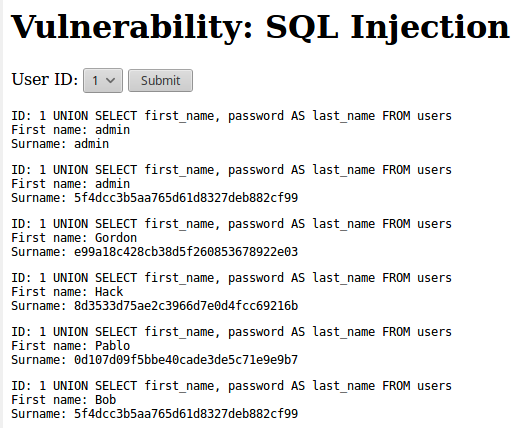
\includegraphics[scale=0.8]{images/sql_injection_medium.png}
    \caption{Captura de pantalla del resultado de la ejecución de la sentencia mostrada en la aplicación \textit{ZAP}}
    \label{fig:sql_injection_medium}
\end{figure}


\subsection{Obteniendo las contraseñas}

Para obtener las contraseñas en texto plano se ha utilizado una herramienta \textit{online\footnote{https://md5hashing.net/hash/md5}} para obtener del texto original dado un \textit{hash MD5}. Por lo tanto si pasamos la herramienta para cada uno de los \textit{hashs} se obtiene la siguiente equivalencia:

\begin{itemize}
    \item \textit{5f4dcc3b5aa765d61d8327deb882cf99} $\rightarrow$ \textit{password}
    \item \textit{e99a18c428cb38d5f260853678922e03} $\rightarrow$ \textit{abc123}
    \item \textit{8d3533d75ae2c3966d7e0d4fcc69216b} $\rightarrow$ \textit{charley}
    \item \textit{0d107d09f5bbe40cade3de5c71e9e9b7} $\rightarrow$ \textit{letmein}
    \item \textit{5f4dcc3b5aa765d61d8327deb882cf99} $\rightarrow$ \textit{password}
\end{itemize}

\newpage

\section{Ataque \textit{SQLi bind}}

Este ataque consiste en la inyección de código \textit{SQL} en el lado del servidor con la dificultad de que ahora es un ataque a ciegas. Ahora la aplicación web no muestra información acerca del resultado de la consulta más allá de la existencia o no de un usuario con el identificador consultado en el sistema.\\
Por lo tanto se han de buscar herramientas adicionales para la explotación de este ataque. La herramienta a utilizar es \textit{SQLMap\footnote{\url{http://sqlmap.org/}}}. Esta herramienta permite explorar las vulnerabilidades de inyección de código \textit{SQL} mediante una serie de tests automáticos. La herramienta se encuentra instalada en la máquina en la ubicación \texttt{/home/dojo/tools/sqlmap/sqlmap.py}.\\


\subsection{Nivel bajo}

Utilizando la herramienta \textit{ZAP} utilizada en el apartado anterior (\ref{section:sqli_medium}) se han obtenido los valores de los campos \textit{cookie} y la \textit{URL} de la petición.\\
La \textit{cookie} está compuesta del identificador \textit{PHPSESSID} que mantiene el estado de la sesión con el servidor y un valor para el atributo \textit{security} que indica la dificultad del reto.\\
Utilizando el siguiente comando sobre el directorio de \textit{sqlmap} y aceptando la ejecución de todos los tests se obtendrá la salida de la Figura \ref{fig:sql_injection_blind_low}. En esta captura se puede observar el sistema gestor de bases de datos con su versión.

\begin{lstlisting}
python sqlmap.py -u "http://dvwa.local/dvwa/vulnerabilities/sqli_blind/?id=1&Submit=Submit" --cookie="security=low; PHPSESSID=ehq3cpfgeqtdg5spr0kaa4isq4"
\end{lstlisting}

\begin{figure}[h!]
    \centering
    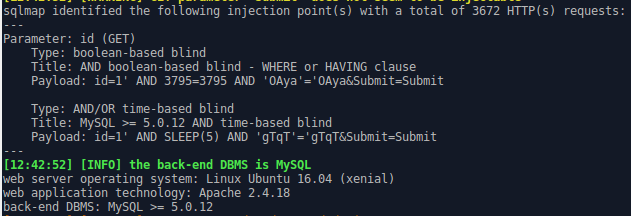
\includegraphics[scale=0.8]{images/sql_injection_blind_low.png}
    \caption{Captura de pantalla de los resultados de la ejecución de la herramienta \texttt{sqlmap} en el nivel de dificultad bajo para el ataque \textit{SQLi Blind}}
    \label{fig:sql_injection_blind_low}
\end{figure}


\subsection{Nivel medio}

En el nivel intermedio pasa algo similar al nivel intermedio de la inyección \textit{SQL} (apartado \ref{section:sqli_medium}). El formulario se ha convertido a un elemento \textit{dropdown} que utiliza el método \textit{POST} para enviar los datos al servidor. Por lo tanto se podría utilizar un método análogo al anterior pero utilizando la opción \texttt{--data} ya que los datos se envían en el cuerpo del mensaje \textit{HTTP POST}.\\
El comando utilizado (desde el directorio \texttt{/home/dojo/tools/sqlmap/}) será el siguiente:

\begin{lstlisting}
python sqlmap.py -u "http://dvwa.local/dvwa/vulnerabilities/sqli_blind/" --cookie="security=medium; PHPSESSID=ehq3cpfgeqtdg5spr0kaa4isq4" --data="id=1&Submit=Submit"
\end{lstlisting}

Los resultados de la ejecución tras aceptar todos los tests se pueden observar en la Figura \ref{fig:sql_injection_blind_medium}.\\

\begin{figure}[h!]
    \centering
    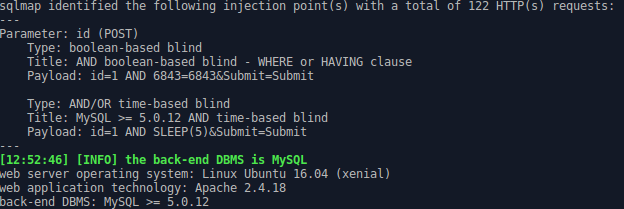
\includegraphics[scale=0.8]{images/sql_injection_blind_medium.png}
    \caption{Captura de pantalla del resultado de la ejecución de la herramienta \texttt{sqlmap} en el nivel de dificultad medio.}
    \label{fig:sql_injection_blind_medium}
\end{figure}


\section{Ataque \textit{CSRF}}

El ataque \textit{CSRF} tiene como objetivo conseguir que los usuarios ejecuten acciones que no querían por medio de envío de peticiones al servidor. Este es un ataque de ingeniería social ya que es necesario que el usuario esté autenticado en el servicio que se pretende atacar y posteriormente interaccione con una web maliciosa, por ejemplo.\\
El objetivo de este ataque será cambiar la contraseña del usuario \textit{admin} sin su consentimiento.\\

\subsection{Nivel bajo}

Para ejecutar el ataque \textit{CSRF} se ha creado una página web que el usuario una vez autentificado en la web original deberá abrir para cambiar su contraseña. El código de la página web es el siguiente:

\lstinputlisting[language=HTML, label={listing:csrf_index.html}]{listings/index-csrf.html}

Esta página realizará una petición \textit{GET} a la web principal enviando las \textit{cookies} de la sesión iniciada del usuario que se haya autentificado. Se puede observar la petición realizada desde la página maliciosa en la Figura \ref{fig:csrf_low}.\\

\begin{figure}[h!]
    \centering
    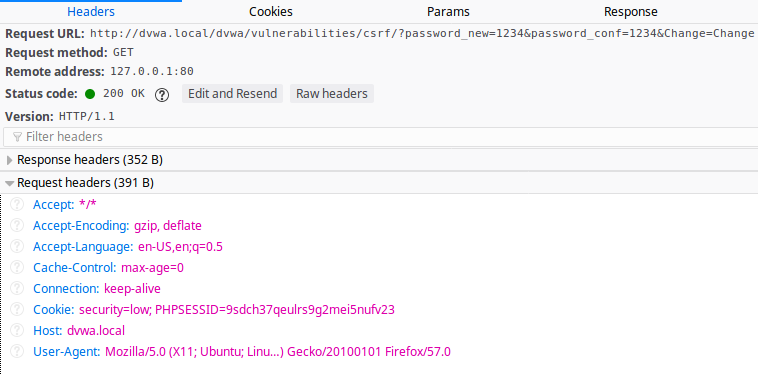
\includegraphics[scale=0.8]{images/csrf_low.png}
    \caption{Captura de pantalla de la petición \textit{GET} desde la página maliciosa para explotar la vulnerabilidad \textit{CSRF}}
    \label{fig:csrf_low}
\end{figure}

Un problema encontrado en la realización de este ataque ha sido que escribiendo la contraseña en el cuadro de texto que se puede encontrar en la página de la vulnerabilidad se recargaba la página y no se mostraba el texto referente al cambio de contraseña y después no permitía iniciar sesión con el usuario \textit{admin}.\\


\subsection{Nivel medio}

En el nivel medio del ataque se ha añadido una comprobación de seguridad adicional: la comprobación del campo \textit{referrer} para evitar los ataques \textit{CSRF}. Con este campo se pretende desechar las peticiones que no son procedentes de la misma web, es decir, se quieren evitar las peticiones \textit{cross-site}. No obstante con esto no se solventa esta vulnerabilidad ya que el campo \textit{referrer} está en la cabecera \textit{HTTP} y se puede modificar utilizando alguna herramienta de captura/emisión de peticiones \textit{HTTP}.\\
En este caso se va a utilizar la herramienta \textit{Burpsuite\footnote{\url{https://portswigger.net/burp}}}, una herramienta con un funcionamiento similar a \textit{ZAP} (utilizada anteriormente). Se ha utilizado esta herramienta porque permite interceptar las peticiones del navegador y modificarlas antes de que se envíen al servidor. Por lo tanto, esta herramienta actúa como un \textit{proxy} y para conseguir que este ataque tenga éxito se debería situar entre el navegador de la víctima y el servidor.\\
Para explotar esta vulnerabilidad se ha activado el proxy en el navegador \textit{Firefox} y en la herramienta se ha activado la opción \textit{Intercept is on} en la pestaña \textit{Proxy}. Una vez están activadas estas opciones se ha vuelto a entrar a la página del Código \ref{listing:csrf_index.html}. Se puede observar que el \textit{Proxy} ha interceptado una petición del navegador (Figura \ref{fig:csrf_medium}).\\

\begin{figure}[h!]
    \centering
    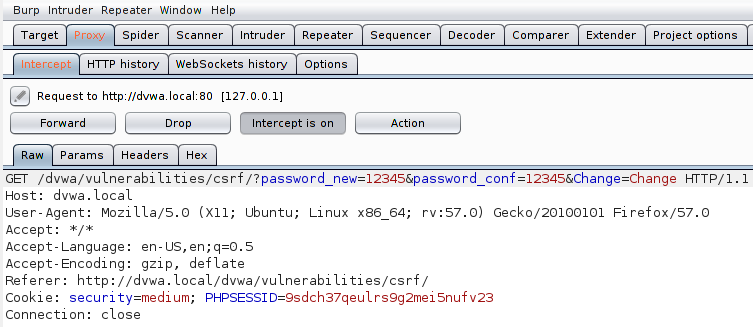
\includegraphics[scale=0.6]{images/csrf_medium.png}
    \caption{Captura de pantalla del \textit{Proxy} en la petición \textit{CSRF}}
    \label{fig:csrf_medium}
\end{figure}

En la Figura anterior se puede observar que se han añadido la cabecera \textit{HTTP} correspondiente al \textit{referrer}. Este debe adoptar el valor de \texttt{http://dvwa.local/dwva/vulnerabilites/csrf} para evitar la contramedida indicada anteriormente.\\
Una vez modificada la petición se pulsará el botón \textit{Forward} para permitir el paso de la petición modificada a través del \textit{Proxy}. La respuesta del servidor es la observada en la Figura \ref{fig:csrf_medium_response}.\\

\begin{figure}[h!]
    \centering
    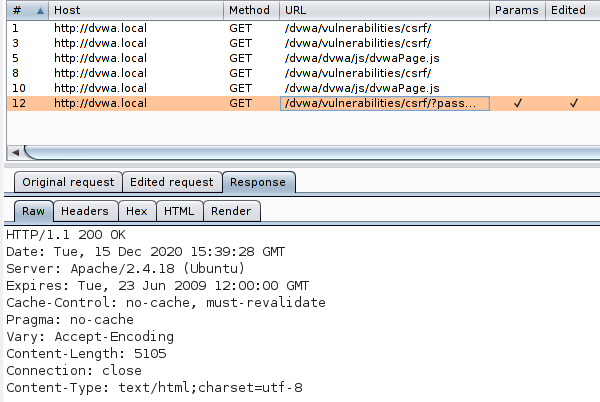
\includegraphics[scale=0.6]{images/csrf_medium_response.png}
    \caption{Captura de pantalla de la respuesta del servidor a la petición modificada con \textit{Burpsuite}}
    \label{fig:csrf_medium_response}
\end{figure}

\newpage
\section{Ataque \textit{XSS (reflected)}}
EL ataque \textit{XSS (reflected)} consiste en realizar una petición \textit{HTTP} al servidor y que este incluye los datos recibidos en la respuesta de forma insegura. De esta manera se puede llegar a ejecutar \textit{scripts} no deseados en el servidor. Para este ataque se pedía obtener las \textit{cookies} de sesión de un usuario.
\subsection{Nivel bajo}
En este nivel, nos encontramos con un formulario que pide al usuario un nombre, a lo que el servidor responde con \texttt{Hello + <nombre>} mediante el comando \texttt{exho} de \textit{PHP}. Para poder realizar el ataque, simplemente se debe de introducir lo siguiente en el formulario:

\begin{lstlisting}
<script> alert(document.cookie) </script>
\end{lstlisting}

De esta manera, el servidor mostrará el contenido del formulario recibido en la petición \textit{GET}, que, como se puede observar es un \textit{script} que muestra las \textit{cookies} de sesión del usuario. Esto es posible ya que el servidor no modifica el contenido del mensaje en ningún momento. Se puede observar el resultado obtenido en la Figura \ref{fig:xss_reflected_low}.

\begin{figure}[h!]
    \centering
    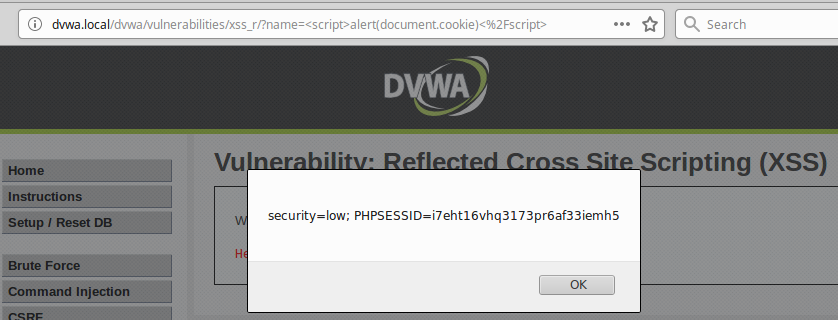
\includegraphics[scale=0.6]{images/xss_reflected_low.png}
    \caption{Captura de pantalla de la respuesta del servidor a la petición con \textit{cookies} de sesión del nivel bajo}
    \label{fig:xss_reflected_low}
\end{figure}

\subsection{Nivel medio}\label{medium-xss-reflected}
En el nivel medio, se comprueba que no haya un tag \texttt{script} en la entrada,por lo que ya no se puede realizar el ataque de la misma manera. Sin embargo, se utilizará otro procedimiento para poder ejecutar código en el lado del servidor. Se introduce el siguiente texto en el formulario:

\begin{lstlisting}
<img src="#" onerror=alert(document.cookie)>
\end{lstlisting}

De esta manera, el servidor ejecutará el código \textit{HTML} con el que se añade un nuevo campo que hace referencia a una imagen. Como la ruta indicada para la imagen (``\#'') no puede ser encontrada por el servidor, se ejecutará el apartado \texttt{onerror}, el cual lanza el \textit{script} utilizado en el nivel anterior. El resultado obtenido es el siguiente:

\begin{figure}[h!]
    \centering
    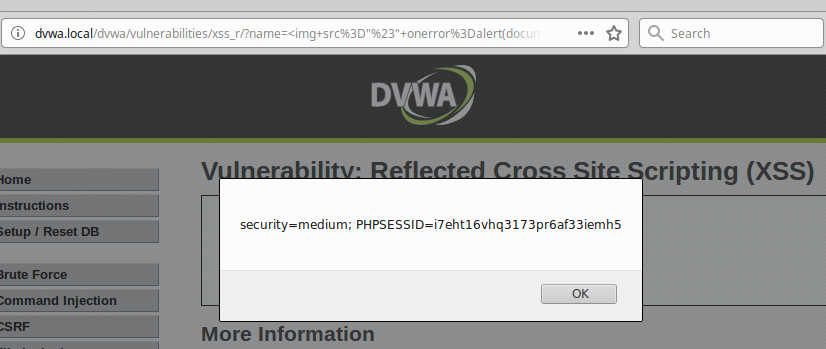
\includegraphics[scale=0.6]{images/xss_reflected_medium.png}
    \caption{Captura de pantalla de la respuesta del servidor a la petición con \textit{cookies} de sesión del nivel medio}
    \label{fig:xss_reflected_medium}
\end{figure}


\section{Ataque \textit{XSS (persistent)}}
El ataque \textit{persistent XSS)} es un tipo de \textit{Cross-Site Scripting} el cual es posible siempre que un servidor web almacene los datos que introduce un usuario y posteriormente se lo muestre a otros usuarios. De esta manera, se puede inyectar código malicioso y almacenarlo en la base del servidor para que repercuta en el resto de usuarios. El objetivo de este ataque es redireccionar a cualquier usuario a una página web elegida por el usuario. La página seleccionada es \url{http://example.org/}.
\subsection{Nivel bajo}
El servidor ofrece al usuario dos formularios, uno para introducir su nombre y otro para escribir un mensaje (máximo 50 carácteres). Tras analizar el código proporcionado, se observa que se sanitizan las entradas, aunque no se evita la introducción de código \textit{HTML}. Por ello, para poder realizar el ataque se debe introducir el siguiente código en el formulario de mensaje \footnote{\url{https://www.w3schools.com/howto/howto_js_redirect_webpage.asp}}: \\

\begin{lstlisting}
<script>location.href="http://example.org"</script>
\end{lstlisting}

Por defecto, este mensaje no puede ser introducido ya que supera el límite de tamaño del campo de \textit{Message}. Para solucionarlo, se accede a \texttt{Inspeccionar elemento}, con lo que se puede modificar el código \textit{HTML} de la página. Se modifica el campo \textit{maxlength} de \textit{mtxMessage}, dándole el valor de 100 en vez de 50. En la Figura \ref{fig:xss_stored_low} se observa todas las modificaciones necesarias para realizar el ataque. \\
\begin{figure}[h!]
    \centering
    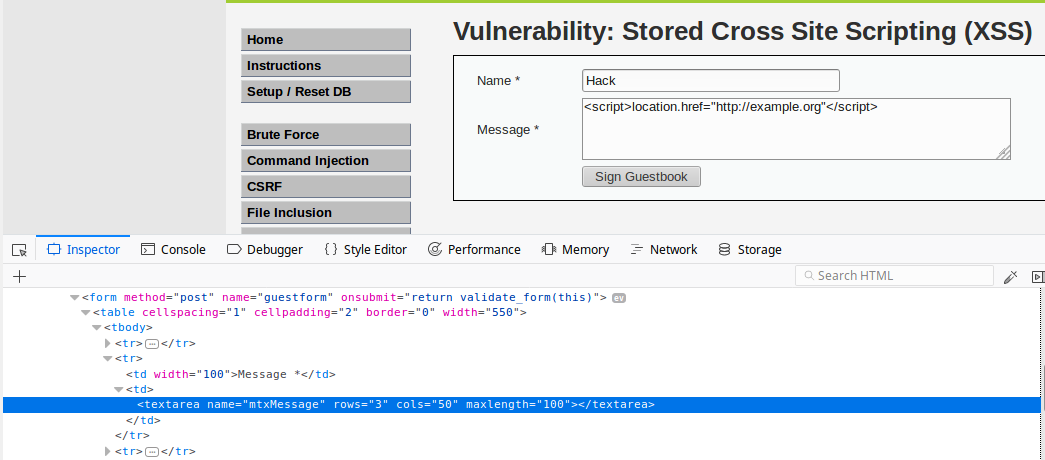
\includegraphics[scale=0.6]{images/xss_stored_low.png}
    \caption{Captura de pantalla de la configuración para realizar el ataque \textit{stored XSS} nivel bajo}
    \label{fig:xss_stored_low}
\end{figure}
\\
Lo que ocurre tras realizar la acción anterior, es que el servidor almacena en la base de datos la información introducida en el formulario. Cuando un usuario accede a este apartado del servicio \textit{WEB}, el servidor muestra todos los mensajes almacenados en la base, por lo que cuando carga el mensaje malicioso, ejecuta el \textit{script} anterior, el cual redirige a la página \url{http://example.org}.
\newpage

\subsection{Nivel medio}

En este nivel, el servidor comprueba en el campo de mensaje que no se esté insertando código \textit{HTML} mediante la función \texttt{strip\_tags()}, mientras que en el campo de \textit{nombre} únicamente se elimina cualquier aparición de \texttt{<script>}. Por ello, nos centraremos en formulario de entrada de \textit{nombre} y realizaremos el ataque mediante el tag de imagen, tal y como se ha comentado en el apartado \ref{medium-xss-reflected}. En este caso, también se debe modificar el campo \textit{maxlength}, ya que está limitado a 30 caracteres. El código a insertar en el campo \textit{nombre} es el siguiente:

\begin{lstlisting}
<img src="#" onerror=location.href="http://example.org">
\end{lstlisting}

Tras ello, el funcionamiento es el mismo que en el del nivel medio. El usuario accede a este apartado, el servidor intenta cargar todos los mensajes almacenados y se ejecuta el \textit{script} maligno que redirige a la página indicada.

\end{document}
